\chapter{Einleitung}
\label{chap:Einleitung}

\section{MyContactCenter}
\label{sec:MyContactCenter}
In vielen Bereichen modernen Lebens hat sich seit dem Anstoß des digitalen Zeitalters ein signifikanter Wandel eingestellt. Das weite Feld  der zwischenmenschlichen Kommunikation zeigt dies wie kaum ein anderes auf. Auch an der Schnittstelle zwischen Privat- und Arbeitsleben zeigt sich diese Modernisierung und im Speziellen an der Kommunikation zwischen Unternehmen und ihren Kunden. Eine moderne Institution dieser Kommunikation ist das Contact Center. Hierbei handelt es sich um einen zentralen Anlaufpunkt für Kunden, an dem diese über verschiedene Kommunikationskanäle ein Anliegen anbringen können, welches von Agenten des Unternehmens bearbeitet wird. Diese Kommunikation ist jedoch nicht einseitig: Auch Contact Center nehmen Kontakt zur Kundschaft auf, um beispielsweise Marktforschung zu betreiben. 
\newline
Laut einer Studie, die 450 Contact Center befragt hat (siehe \cite{Deloitte:17}), werden die Kommunikationsanforderungen von modernen Contact Centern nicht nur umfangreicher, sondern auch komplexer. Die von der Firma ilogixx hergestellte Software-Lösung MyContactCenter (im Folgenden mit MyCC abgekürzt) hat zum Ziel, Betreiber von Contact Centern dabei zu unterstützen, diese wachsenden Anforderungen zu erfüllen. Dafür stellt das Produkt einem Contact Center Werkzeuge zur Verfügung, die die Effizienz bei der Bearbeitung von Kundenanfragen erhöhen. Ein solches Werkzeug und eine Kernaufgabe des Produktes ist die Automatische Kontakt Verteilung (kurz ACD für ``automatic contact distribution''). Das Produkt nimmt hierbei Anfragen auf unterschiedlichen Kommunikationskanälen entgegen, kategorisiert diese nach Sprache und Aufgabenbereich, und teilt sie freien Agenten zu, welche für diese Aufgabenbereiche beziehungsweise Sprache eingeteilt sind. Die Agenten interagieren nun über MyCC mit dem Anfragenden, bis die Kommunikation auf beiden Seiten beendet wird. Anschließend hat der Agent eine Nachbearbeitungszeit, in der das Anliegen des Anfragenden zu Ende gebracht werden kann. Danach ist der Agent wieder für die nächste Anfrage frei.
\newline
MyContactCenter ist eine verteilte Anwendung. Die Hauptkomponente ist der Server, welcher den Großteil der Verwaltungsaufgaben übernimmt. Er verwaltet eine Liste der angemeldeten Agenten, sowie deren aktuellen Kommunikationsstatus (frei, im Gespräch, etc.) und Nutzerdaten (Name, Sprache, Wissensbereich, etc.). Auch Kategorisieren und Zuordnen von Anfragen während der automatischen Kontakt Verteilung und das Weiterleiten selbiger an den nächsten freien Agenten gehört zu seinen Aufgaben. Konfiguriert wird der Server über einen Administrations-Client. Hier kann der Administrator des Contact Centers alle für den Betrieb benötigten Einstellungen vornehmen, wie zum Beispiel das Anlegen von neuen Sprachen und Wissensbereichen, oder das Verwalten von Agenten-Daten. Agenten besitzen eine eigene Client-Anwendung, die sich für die Dauer der Nutzungszeit am Server anmeldet.  Mit diesem Client kann der Agent vom Server erhaltene Anfragen bearbeiten, also zum Beispiel eine Email beantworten oder sein IP-Telefon, auch Soft Phone genannt, steuern. Das Soft Phone steht in Verbindung mit der Software-Telefonanlage, auch PBX (Private Branch Exchange) genannt, die die eigentliche Voice Over Ip-Technologie realisiert. Die PBX steht in Verbindung mit dem MyCC-Server und tauscht über TCP Nachrichten aus, wie zum Beispiel welcher Agent als nächstes angerufen werden soll etc. In Abbildung \ref{fig:MyCCStructure} sind die einzelnen Komponenten von MyContactCenter dargestellt.
\newline
In Version zehn von MyContactCenter kommt eine wichtige Komponente hinzu: Die Routing Engine. Diese nimmt eingehende Anrufe auf Ebene des Session Initiation Protocol (SIP) entgegen und kommuniziert an Stelle des MyCC-Servers mit der PBX. Abbildung \ref{fig:InteractionIncomingCall} stellt den Kommunikationsablauf im Falle eines eingehenden Anrufes dar. Ruft ein Kunde das Contact Center an, wird über den sogenannten Trunk die Schnittstelle zwischen dem ISDN-Telefonnetz und der PBX hergestellt. Die PBX nimmt den Ruf an und baut eine Verbindung zur Routing Engine auf. Ist die Sitzung erfolgreich hergestellt, kann der Medienstrom über das Real Time Protocol (RTP) zwischen der Routing Engine und dem Trunk, welche die Medien an den Anrufer weiterleitet, ausgetauscht werden. Im nächsten Schritt kann die Routing Engine, falls gewünscht, nun den Ruf an einen Agenten durchstellen, beispielsweise über eine Warteschleife. Dafür hält die Routing Engine über eine TCP-Verbindung Rücksprache mit dem MyCC-Server und schickt die Anweisung, den aktuellen Ruf in eine Warteschleife zu platzieren. Der Server antwortet mit dem nächsten freien Agenten, dem der Ruf zugeteilt werden soll. Anschließend wird über die PBX eine Sitzung zwischen dem Agenten und der Routing Engine ausgehandelt. Die Routing Engine verschmilzt nun beide Medienströme, sodass die Medien des Agenten beim Anrufer ankommen und umgekehrt. 
\newline
Die Routing Engine hat eine hohe Kontrolle darüber, wie mit einem eingehenden Anruf umgegangen wird. So kann zum Beispiel neben dem Zustellen ein Anruf alternativ sofort aufgelegt werden. Auch die Manipulation des Medienstroms zwischen Anrufer und Agent ist denkbar. Damit die Benutzer von MyContactCenter von der Flexibilität der Routing Engine profitieren können, wird eine Möglichkeit benötigt, ihr Verhalten möglichst detailliert zu konfigurieren. Die vorliegende Ausarbeitung beschäftigt sich zu diesem Zweck mit dem Entwurf und der Implementierung einer domänenspezifischen Sprache, die es den Benutzern von MyContactCenter ermöglicht, das Verhalten der Routing Engine frei zu programmieren.   

\begin{figure} %[hbtp]
	\centering
		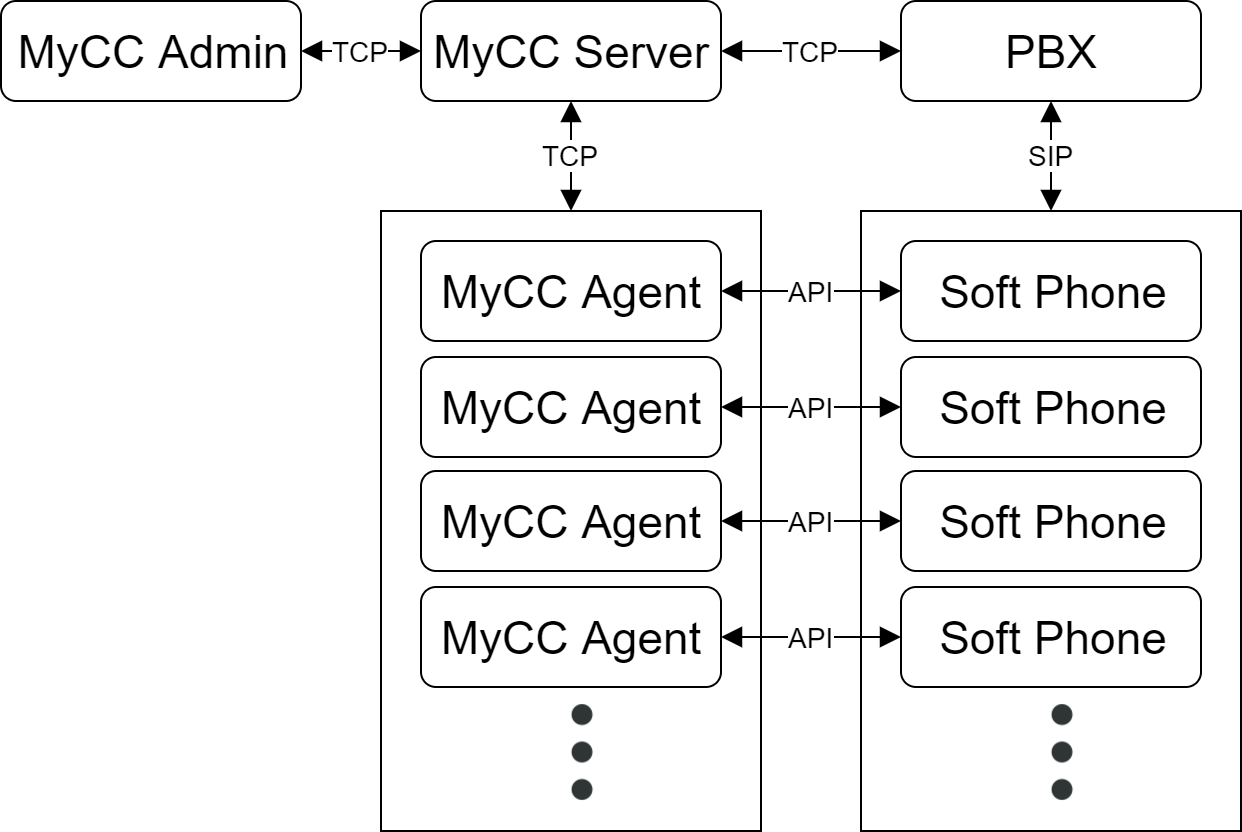
\includegraphics[width=\textwidth]{img/MyCCStructure.png}
	\caption[Komponententstruktur von MyContactCenter]{Die Komponenten von MyContactCenter und wie sie miteinander in Verbindung stehen. Der MyCC-Server übernimmt eine zentrale Rolle und verwaltet die Agenten- und Admin-Clients, die über TCP mit ihm in Verbindung stehen. Die eigentliche Voice-Over-IP-Infrastruktur wird über eine PBX realisiert, an welcher die Softphones der Agenten angebunden sind. Die Schnittstelle zwischen MyCC und der PBX ist auf der Server-Seite eine TCP-Verbindung, über die Nachrichten ausgetauscht werden, und auf der Client-Seite eine API, über die der MyCC-Agent mit dem Softphone kommuniziert.}
	\label{fig:MyCCStructure}
\end{figure}

\begin{figure} %[hbtp]
	\centering
		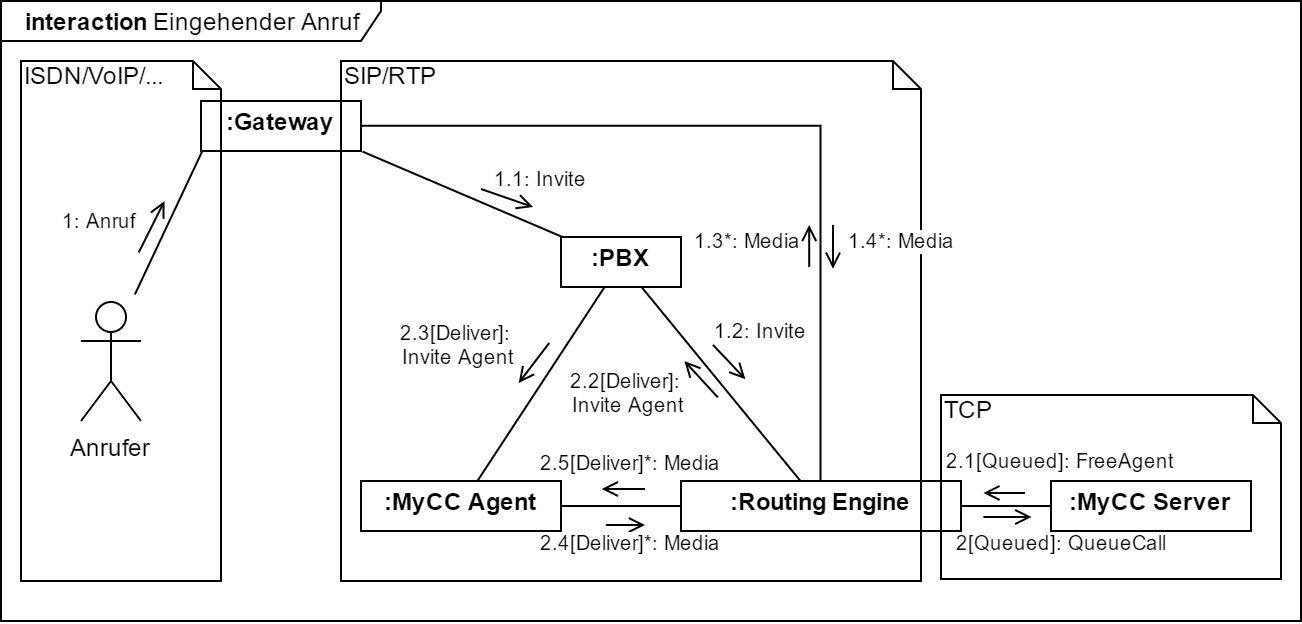
\includegraphics[width=\textwidth]{img/RoutingEngineSipExplanation.png}
	\caption[Behandlung eingehender Rufe in MyContactCenter]{Behandlung eingehender Anrufe in MyContactCenter.}
	\label{fig:InteractionIncomingCall}
\end{figure}
 
\newpage
 
\section{Motivation}
\label{sec:Motivation}
Die Motivation des vorliegenden Projektes soll zum Einstieg mit folgenden User-Stories eingeleitet werden:
\begin{itemize}
\item Als Administrator möchte ich vor dem Zustellen eines Kundenrufes eine Begrüßung abspielen.
\item Als Administrator möchte ich vor dem Zustellen eines Kundenrufes per Frequenzwahlverfahren abfragen, welche Sprache der Anrufer spricht.
\item Als Administrator möchte ich bei eingehenden Anrufen außerhalb der Ge\-schäftszeiten den Ruf ablehnen.
\item Als Administrator möchte ich bei einer eingehenden Email eine Vorlage als Standard-Antwort verschicken.
\end{itemize}
Den oben aufgelisteten Anforderungen ist nicht nur die eingenommene Kundenrolle des Administrators gemeinsam. Auch die zu erreichenden Ziele ähneln sich: Die Behandlung einer eingehender Kontaktanfrage durch die Software soll vom Kunden konfigurierbar sein. Dabei soll dem Kunden größtmögliche Freiheit geboten werden, um möglichst viele Anforderungen eines Contact Centers abzudecken. Zu den oben stehenden User-Stories können demnach noch zahlreiche weitere Beispiele mit ähnlichem Muster konstruiert werden. Die Software MyContactCenter hat den Anspruch all diesen Anforderungen gerecht werden, um in möglichst vielen Contact Centern Anwendung finden zu können. Der so resultierende Grad an individueller Konfiguration der Software durch den Anwender ist hoch. Das Problem wird bewältigt, indem es dem Benutzer möglich gemacht wird, das Verhalten von MyContactCenter im Falle einer Kontaktanfrage selber zu programmieren. Als Mittel dazu wird eine eigene grafische domänenspezifische Programmiersprache angeboten, deren Entwicklung und Implementierung Hauptgegenstand der vorliegenden Arbeit ist.
\newline
Für MyContactCenter als Software-Produkt ergibt sich aus diesem Vorgehen eine Reihe von Vorteilen:

\begin{description}
\item[Flexible Konfiguration] \hfill \\
Der Anwender erhält erhöhte Kontrolle über das Conversation Routing in seinem Contact Center. Die Features, die in der neuen DSL angeboten werden (das Abspielen von Audiodateien etc.) sind zwar nicht neu. Aber nun kann flexibler auf diese zugegriffen werden und mehr Anforderungen von Contact Centern können erfüllt werden.
\item[Unabhängigkeit gegenüber Drittanbietern] \hfill \\
Vor der Implementierung der DSL lief das Conversation Routing über die PBX ab: Eingehende Anrufe wurden über eine Scripting-Schnittstelle der Telefonanlage geroutet. Mit einer eigenständigen DSL erhält MyCC eine neue Unabhängigkeit gegenüber den Beschränkungen und Nachteilen solcher Drittanbieter-Software.
\item[Hohe Skalierbarkeit] \hfill \\
Die Ausführung von DSL-Skripten wird von einem dediziertem Dienst, der Routing Engine, übernommen. Dies entlastet den MyCC-Server und erlaubt das parallele Aufschalten von mehreren Conversation Routing Engines bei hoher Systemlast. So kann die generelle Performanz von MyCC verbessert werden.
\end{description}

\section{Domänenspezifische Sprachen}
Bei domänenspezifischen Sprachen handelt es sich um formale Sprachen, die es einem menschlichen Benutzer ermöglichen, Berechnungsvorschriften zu spezifizieren. In diesem Punkt ähneln sie prominenten Programmiersprachen wie C oder Java. Anders als diese Universalsprachen (engl. General Purpose Languages), welche Turing-vollständig sind, werden DSLs jedoch mit Absicht mit beschränktem Anwendungsgebiet designt. Ihre Anwendung beschränkt sich auf das Lösen von Problemen aus einer bestimmten Domäne. Diese Domänen können vielfältig sein: Beispiele sind hier das Steuern von Kühlschränken, das Spezifizieren von Benutzeroberflächen von Handy-Anwendungen oder das Beschreiben von Versicherungspaketen (siehe \cite[S. 93ff.]{Kelly:08}. Besondere Beachtung finden DSLs in der modellgetriebenen Softwareentwicklung (engl. Model Driven Devlopment oder MDD), welche zum Ziel hat, Software nicht mehr über herkömmlichen, von Hand geschriebenen Programmiercode zu entwickeln. Stattdessen wird Software in Form von Modellen spezifiziert, welche in einer (oftmals eigens für das Problem zur Hand entworfenen) DSL vorliegen. Diese Modelle werden als Vorlage genommen, um daraus ausführbaren Code, oft in einer  Universalsprache, zu generieren \cite[S. 29]{Voelter:13}. Dies wird als Transformation bezeichnet. Der Fokus beim Model Driven Development also liegt nicht mehr auf dem Quellcode selbst, sondern auf Modellen, welche das Verhalten der Software spezifizieren. Befürworter von domänenspezifischen Sprachen loben den Einsatz von dieser als Mittel, um die Qualität der entstehenden Software und die Produktivität des Herstellungsprozesses zu erhöhen \cite[S. 33f]{Fowler:11}. Die Transformation von einem DSL-Modell in den Code einer maschinennäheren Programmiersprache sei vergleichbar mit dem Sprung auf höhere Abstraktionsstufen, der vollzogen wird, wenn Programmiersprachen einen Generationswechsel vollziehen. Damit einher gingen die verbundenen Vorteile bei der Softwareentwicklung \cite[S. 15ff]{Kelly:08}.
\newline
In der vorliegenden Arbeit wird eine domänenspezifische Sprache nicht im Zuge von modellgetriebener Softwareentwicklung eingesetzt. Zwar wird auch eine Transformation auf Modelle der DSL angewandt. Aber der Zweck dient nicht der Entwicklung, sondern der Konfiguration von MyContactCenter. Eine domänenspezifische Sprache bietet sich für diese Aufgabe aus folgenden Gründen an: 
\begin{description}
\item[Modellierung statt Programmierung] \hfill \\
Bei der Zielgruppe der DSL handelt es sich nicht um Programmierer, sondern um Anwender von MyContactCenter. Die Anwender sind also versiert im Betreiben eines Contact Centers und verfügen damit ein breites Wissen über die Domäne: Das Routing von Konversationen in Contact Centern. Es handelt sich um sogenannte Domänenexperten (engl. domain experts). Es kann jedoch nicht davon ausgegangen werden, dass Domänenexperten über Programmierkenntnisse mit Universalsprachen verfügen. Würde eine solche Universalsprache zum Einsatz kommen, bestünde ein Risiko, dass ein großer Teil der Zielgruppe aufgrund von fehlender Qualifizierung und Verständnis das Produkt nicht nutzen kann. Ebenso werden Anwender vor fehlerhafter Programmierung geschützt. Dies ist auch der Grund, warum eine grafische und keine textuelle DSL zum Einsatz kommt: Grafische Repräsentationen gelten laut \cite[S. 50f]{Kelly:08} als ausdrucksstärker, verständlicher und weniger fehleranfällig.
\item[Domänenspezifische Einschränkung] \hfill \\
Die Anzahl an unterschiedlichen Möglichkeiten zur Konfigurierung des Konversationsroutings rechtfertigt deren Programmierbarkeit. Dennoch muss hier keine Turing-vollständige Programmierung stattfinden. Durch die Einschränkung auf eine Domäne profitiert der Anwender von den Vorteilen die domänenspezifische Sprachen zugeschrieben werden: Weniger Fehler mit aussagekräftigeren Fehlermeldungen, sicherere und leichter zu analysierende Programme sowie leichtere Erlernbarkeit \cite{Tomassetti:17}.
\item[Verbesserte Kommunikation] \hfill \\
Als Benutzer von MyContactCenter stehen die Anwender der DSL häufig in Kontakt mit dem Hersteller (beispielsweise im Zuge von technischem Support oder bei Verkaufsgesprächen). In diesen Austäuschen ist eine eindeutige Kommunikation wichtig, auch wenn es um das Routing von Konversationen geht. Die grafischen Modelle der DSL stellen eine unmissverständliche Dokumentation der Spezifikation solcher Konversationsroutings dar, die sowohl aus Entwickler- als auch aus Domänenexpertensicht verständlich ist. Auf diese Weise trägt die DSL zur erfolgreichen Kommunikation zwischen Anwendern und Hersteller bei.
\end{description}


\section{Benötigtes Vorwissen}
MyContactCenter kommt in einem umfangreichen Ökosystem von Drittanbieter-Software zum Einsatz. Für das weitere Verständnis der vorliegenden Arbeit werden die Prinzipien einiger Technologien erläutert, welche Einfluss auf die Implementierung der domänenspezifischen Sprache nehmen. 

\subsection{.NET}
MyContactCenter und die DSL ist mit dem Microsoft .NET Software Framework entwickelt worden. Hauptbestandteile von .NET ist die Microsoft Intermediate Language (MSIL), auch genannt Common Intermediate Langugage (CIL), und die Common Language Runtime (CLR), welche Sprachinteroperabilität zwischen unterschiedlichen Universalsprachen (wie zum Beispiel C\# oder Visual Basic) ermöglicht. Benutzer des .NET Frameworks schreiben Code in einer vom Framework unterstützen Sprache, welcher vom Compiler in vom Menschen größtenteils unlesbaren MSIL-Bytecode übersetzt wird. Dieser Bytecode wird von der CLR mittels eines Just-In-Time-Compilers in Maschinencode transformiert und ausgeführt (vgl. \cite[S. 16ff]{Platt:03}). Zusätzlich stellt das .NET Framework eine große Anzahl an Bibliotheken mit grundlegenden Funktionen zur Verfügung. 

\subsection{Roslyn}
Roslyn ist eine .NET Compiler-Plattform welche Entwicklern die Werkzeuge eines Compilers für C\#- und Visual Basic-Code über eine API im eigenen Programmcode zur Verfügung stellt. So kann Code von Dritt-Anwendungen analysiert, generiert und kompiliert werden (siehe dazu den frei zugänglichen Quellcode und die Dokumenation \cite{Roslyn}). Die Implementierung der domänenspezifischen Sprache benutzt Roslyn um über eine Codegenerierungs-API einen MSIL-Syntaxbaum zu generieren und diesen zu einem .NET-Assembly zu kompilieren. Über die API können einem bestehenden Syntaxbaum neue Syntaxknoten hinzugefügt werden, welche sich nach den Regeln der Microsoft Intermediate Language schachteln lassen. Syntaxknoten und -Bäume sind unveränderlich (engl. immutable), das heißt wenn ein Syntaxbaum einmal angelegt ist, kann dieser nicht mehr verändert, sondern nur noch kopiert werden. In der vorliegenden Ausarbeitung wird der Syntaxbaum mit Roslyn daher ''Bottom-up`` generiert: Anstatt zuerst den Syntaxbaum zu instanzieren und anschließend die Knoten und Baumblätter hinzuzufügen, werden zuerst die Blätter und Knoten erzeugt, welche nacheinander zu einem Baum zusammengesetzt werden. 
\newline
Sei beispielsweise die Syntax für folgenden Code zu generieren:
\newline
\vspace{1cm}
\noindent
\begin{minipage}{1.0\textwidth} \small
\begin{lstlisting}
public class RoslynTest
{
    public int Return5()
    {
        return 2 + 3;
    }
}
\end{lstlisting}
\end{minipage}
\vskip 1em
Dann ließe sich dies durch folgenden Code-Ausschnitt realisieren:
\newline
\vspace{1cm}
\noindent
\begin{minipage}{1.0\textwidth} \small
\begin{lstlisting}
var workSpace = new AdhocWorkspace();

var generator = SyntaxGenerator(workSpace, LanguageNames.CSharp);

var literal2 = generator.LiteralExpression(2);

var literal3 = generator.LiteralExpression(3);

var addExpression = generator.AddExpression(literal2, literal3);

var returnStatement = generator.ReturnStatement(addExpression);

var returnType = generator.TypeExpression(SpecialType.System_Int32);

var methodDeclaration = generator.MethodDeclaration("Return5", null, null, returnType, Accessibility.Public, DeclarationModifiers.None, returnStatement);

var methodDeclarationArray = new SyntaxNode[] { methodDeclaration };

var classDeclaration = generator.ClassDeclaration("RoslynTest", null, Accessibility.Public, DeclarationModifiers.None, null, null, methodDeclarationArray);

var classDeclarationArray = new SyntaxNode[]{ classDeclaration };

var syntaxTree = generator.CompilationUnit(classDeclarationArray).SyntaxTree;
\end{lstlisting}
\end{minipage}
\vskip 1em

\subsection{Asynchrone Methodenausführung in .NET}
\label{subsec:Asynchrone Methodenausfuehrung}
Einige Operationen innerhalb eines Konversationsroutings erfordern Thread-blockierende Operationen (zum Beispiel das Abspielen von Audiodateien). Um solche Blockaden zu verhindern, werden diese mittels asynchroner Methodenausführung auf anderen Threads ausgeführt. Dies findet in .NET über eine das Async/Await-Sprachkonstrukt statt, welches anhand des unten stehenden Codes erklärt werden soll.

\vspace{1cm}
\noindent
\begin{minipage}{1.0\textwidth} \small
\begin{lstlisting}
async Task<int> A ()
{
	int temp = await B();
	return temp;
}

Task<int> B ()
{
	return Task.Run<int>( () => DoWork() );
}
\end{lstlisting}
\end{minipage}
\vskip 1em


Eine Methode, hier genannt Methode A, kann mit dem Schlüsselwort ``async'' gekennzeichnet werden. Dies signalisiert, dass A eine asynchrone Methode ist, welche in ihrem Methoden-Körper mittels des ``await''-Schlüsselworts auf die andere Methode B warten kann. Trifft der Programmfluss auf dieses ``await'', wird die Kontrolle an den Aufrufer von A zurückgegeben, während auf das Ergebnis von B gewartet wird. Der Aufrufer von A kann nun mit seiner Arbeit weiter machen, oder gemäß des Musters mittels ``await'' auf A warten. Bs Arbeit wird mit der Methode ``Task.Run'' gestartet, welche die zu verrichtende Arbeit auf einem anderen Thread startet und ein Task-Objekt zurückliefert. Ist der Thread mit seiner Arbeit fertig (in diesem Fall mit der Methode ``DoWork'') wird das Ergebnis in dem Task-Objekt gespeichert, von dem ``await''-Operator abgeholt, und in die Variable ``temp'' geschrieben. ``temp'' wird nun zurückgeliefert, was bedeutet, dass der von A zurückgelieferte Task nun das gewünschte Ergebnis enthält. Auf diese Weise wurde der Hauptprogrammfluss nicht blockiert, obwohl eine potentiell rechenintensive Operation in B ausgeführt wurde.


\subsection{SIP}
Die Kommunikation der Routing Engine mit der PBX findet über das Session Initiation Protocol statt. Es handelt sich hierbei um ein Klartext-Protokoll, welches in der Anwendungsschicht des OSI-Modells angesiedelt ist. Es wird dafür benutzt, Kommunikationssitzungen zwischen sogenannten User Agents zu initiieren. Solche User Agents können beispielsweise Soft-Phones sein, die an der PBX angemeldet sind. Die PBX agiert im Kontext von SIP als Proxy-Server, welcher die Vermittlung zwischen User Agents sicherstellt. Ist eine Kommunikationssitzung zu Stande gekommen, wird ein Medienstrom über das Real-Time Transport Protocol ausgetauscht. Die Conversation Routing Engine, also der Teil von MyContactCenter, der die DSL-Modelle ausführt, ist als User Agent an der PBX angemeldet und der Sitzungspartner einer eingehenden Konversation während des Verlaufs eines Konversationsroutings. Die Implementierung des Session Initiation Protocols ist an einer Drittanbieter-Bibliothek namens PJSIP ausgelagert. Diese übernimmt auch die Implementierung eines SIP User Agents. 

\subsection{Protocol Buffers}
Protocol Buffers sind eine von Google entwickelte Methode, um Daten zu serialisieren. Im hier beschriebenen Projekt wird eine Implementierung dessen namens Protobuf verwendet, um DSL-Strukturen als Bytestrom zwischenzuspeichern und zu übermitteln. Gegenüber Klartext-Verfahren wie XML oder JSON bietet Protobuf einen Performance-Vorteil (siehe \cite{Bowden:14}).

\subsection{Windows Forms und Devexpress}
Die grafische Benutzeroberfläche von MyCC und damit auch des grafischen DSL-Editors ist mit der Windows Forms-Technologie implementiert. Dabei handelt es sich um eine .NET-Bibliothek die Werkzeuge zum Designen und Darstellen von grafischen Benutzeroberflächen zur Verfügung stellt. Obwohl es neuere Frameworks zur Entwicklung von grafischen Benutzeroberflächen gibt (zum Beispiel die Windows Presentation Foundation), werde Windows Forms laut Microsoft weiterhin unterstützt und gewartet (siehe \cite{Allen:14}). Programme die Windows Forms verwenden, benutzen zur Interaktion mit der Benutzeroberfläche .NET Events \cite[S. 171ff]{Platt:03}. Das heißt, dass die grafische Benutzeroberfläche aus Komponenten (sog. Controls) zusammengestellt wird, welche bei Interaktion durch einen Benutzer Events auslösen, auf die zu Grunde liegender Code dann reagieren kann. Zur Ergänzung von Windows Forms wird in der vorliegenden Arbeit die Drittanbieter-Bibliothek Devexpress verwendet, welche Erweiterungen vor allem in Form von komplexen Controls zur Verfügung stellt. 